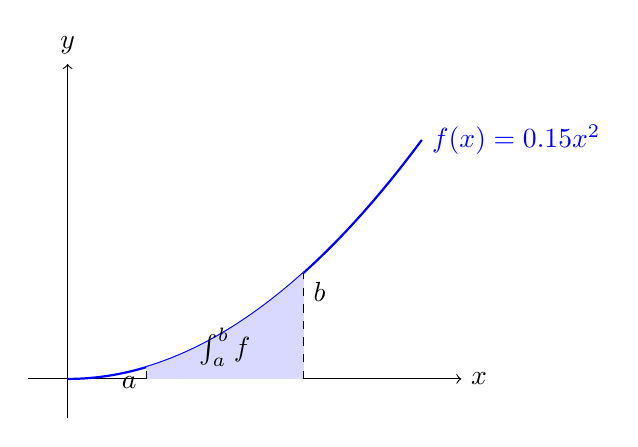
\begin{tikzpicture}
    % Axes
    \draw[->] (-0.5,0) -- (5,0) node[right] {$x$};
    \draw[->] (0,-0.5) -- (0,4) node[above] {$y$};

    % Curve
    \draw[blue, thick, domain=0:4.5, samples=100]
        plot (\x, {0.15*\x*\x}) node[right] {$f(x) = 0.15x^2$};

    % Filled area
    \fill[blue!15, domain=1:3, samples=50]
        (1,0) -- plot (\x, {0.15*\x*\x}) -- (3,0) -- cycle;

    % Bounds
    \draw[dashed] (1,0) -- (1,0.15) node[below left] {$a$};
    \draw[dashed] (3,0) -- (3,1.35) node[below right] {$b$};

    % Label
    \node at (2,0.4) {$\int_a^b f$};
\end{tikzpicture}
